
%(BEGIN_QUESTION)
% Copyright 2010, Tony R. Kuphaldt, released under the Creative Commons Attribution License (v 1.0)
% This means you may do almost anything with this work of mine, so long as you give me proper credit

Suppose we have a Siemens S7-200 PLC connected to a pair of momentary-contact pushbutton switches and light bulbs as shown in this illustration:

$$\includegraphics[width=15.5cm]{i04170x01.eps}$$

Examine the following relay ladder logic (RLL) program for this Siemens PLC, determining the statuses of the two lamps provided switch A is pressed by a human operator and switch B is unpressed:

$$\includegraphics[width=15.5cm]{i04170x02.eps}$$

Furthermore, determine whether the inputs and outputs of this particular PLC (as shown) are {\it sourcing} or {\it sinking}.

\underbar{file i04170}
%(END_QUESTION)





%(BEGIN_ANSWER)

Hint: to identify whether an I/O point is sourcing or sinking, sketch arrows showing the direction of electric current (using conventional flow notation) where wires connect to the I/O channel terminals.  If the arrow shows current {\it exiting} the PLC channel and headed toward an external device, then that I/O channel is {\it sourcing} current to that device.  If the arrow shows current {\it entering} the PLC channel from an external device, then that I/O channel is {\it sinking} current from that device.

%(END_ANSWER)





%(BEGIN_NOTES)

Output {\tt Q0.3} will activate to energize lamp Z, but the other output (and lamp) will remain off. 

\vskip 10pt

The inputs on this Siemens S7-200 PLC are {\bf sinking}, while the outputs are {\bf sourcing}.




\vfil \eject

\noindent
{\bf Prep Quiz:}

Determine the statuses of the blue and yellow lamps, assuming pushbuttons A and B are being pressed, and pushbutton C is not.  Note that this is an ``offline'' display of the PLC's program, where no status highlighting is shown:

$$\includegraphics[width=15.5cm]{i04170x03.eps}$$

\vfil \eject

\noindent
{\bf Prep Quiz:}

Determine the statuses of the blue and yellow lamps, assuming pushbuttons A and C are being pressed, and pushbutton B is not.  Note that this is an ``offline'' display of the PLC's program, where no status highlighting is shown:

$$\includegraphics[width=15.5cm]{i04170x03.eps}$$

\vfil \eject

\noindent
{\bf Prep Quiz:}

Determine the statuses of the blue and yellow lamps, assuming pushbuttons B and C are being pressed, and pushbutton A is not.  Note that this is an ``offline'' display of the PLC's program, where no status highlighting is shown:

$$\includegraphics[width=15.5cm]{i04170x03.eps}$$




%INDEX% PLC, relating I/O status to virtual elements

%(END_NOTES)


